\section{公差分析}

\subsection{公差分析的意义}

光学设计的最终目的是指导实际加工生产。理论上的最优设计在实际制造中必然存在各种加工误差，公差分析的目的是评估这些制造误差对最终成像质量的影响，并制定合理的加工公差范围，在保证像质的前提下尽量降低加工难度和成本\cite{Smith2008,Born1999,Fischer2008}。

现代光学元件的主要加工误差来源包括：透镜曲率半径的加工公差、镜片厚度的加工公差、玻璃折射率和阿贝数的材料误差、各透镜之间的偏心误差和倾斜误差，以及装配引入的综合误差。

\subsection{公差设置}

在Zemax的Tolerance Data Editor中，依据实际光学加工的工业水平，设置如下公差范围\cite{Fischer2008,Zemax2021}：

表6.1 公差设置参数表

\begin{longtable}[]{@{}
  >{\raggedright\arraybackslash}p{(\columnwidth - 8\tabcolsep) * \real{0.1551}}
  >{\raggedright\arraybackslash}p{(\columnwidth - 8\tabcolsep) * \real{0.2909}}
  >{\raggedright\arraybackslash}p{(\columnwidth - 8\tabcolsep) * \real{0.2216}}
  >{\raggedright\arraybackslash}p{(\columnwidth - 8\tabcolsep) * \real{0.1773}}
  >{\raggedright\arraybackslash}p{(\columnwidth - 8\tabcolsep) * \real{0.1551}}@{}}
\toprule\noalign{}
\endhead
\bottomrule\noalign{}
\endlastfoot
\textbf{公差类型} & \textbf{含义} & \textbf{公差范围} & \textbf{灵敏度排序} & \textbf{是否关键} \\
TRAD & 曲率半径误差（面1\textasciitilde6） & ±0.05 mm & 较高 & 是 \\
TTHI & 镜片中心厚度误差 & ±0.05 mm & 中等 & 是 \\
TIND & 折射率误差 & ±0.001 & 中等 & 是 \\
TABB & 阿贝数误差 & ±0.5\% & 低 & 否 \\
TEDX\/\allowbreak TEDY & 透镜偏心误差（X/Y方向） & ±0.05 mm & 高 & 是 \\
TETX\/\allowbreak TETY & 透镜倾斜误差（X/Y方向） & ±0.05° & 高 & 是 \\
\end{longtable}

上述公差范围基于一般光学冷加工水平设定。对于高精度产品，曲率半径和偏心公差可进一步收紧至±0.01 mm级别。公差的具体数值应根据蒙特卡洛分析的良品率结果进行迭代调整。

\subsection{灵敏度分析}

在蒙特卡洛分析之前，首先进行灵敏度分析（Sensitivity Analysis）。灵敏度分析对每个公差因子单独施加最大误差，计算其对评价指标（RMS波前误差）的影响量，从而找出对像质影响最大的关键误差源。

通常，透镜倾斜（TETX\/\allowbreak TETY）和偏心（TEDX\/\allowbreak TEDY）对成像质量的影响较大，是需要重点控制的公差因子。曲率半径公差（TRAD）次之，折射率公差（TIND）的影响相对较小。

\begin{figure}[H]
  \centering
  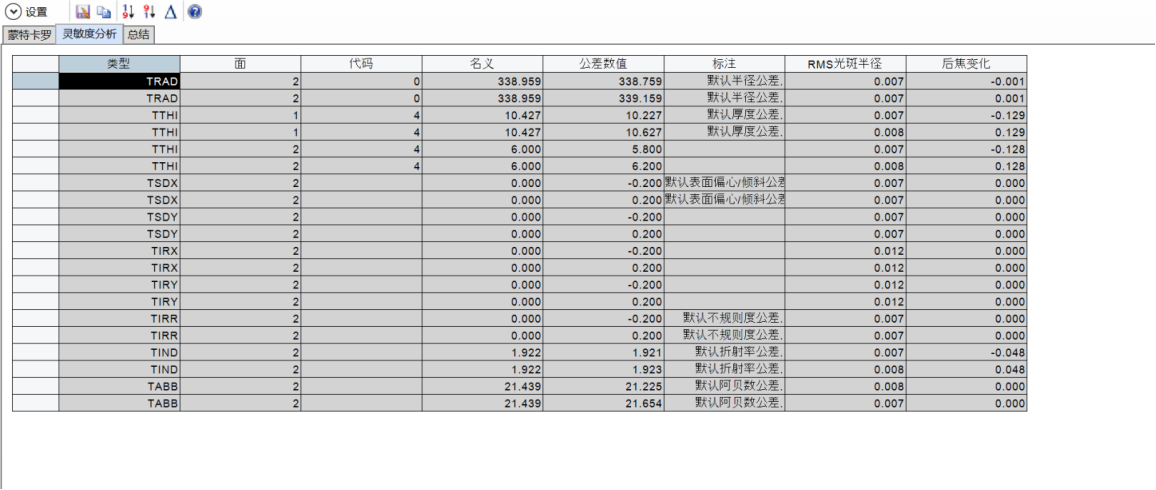
\includegraphics[width=0.95\textwidth]{chapters/chapter6/figures/Sensitive.png}
  \caption{灵敏度分析结果（各公差因子对RMS波前误差的贡献）}
  \label{fig:chapter6-sensitive}
\end{figure}

\subsection{蒙特卡洛分析}

采用蒙特卡洛（Monte Carlo）方法进行统计公差分析。在设定的公差范围内随机生成500个样本（每个样本对应一组随机的制造误差组合），对每个样本计算RMS波前误差，最终给出像质指标的统计分布，并计算满足设计要求（RMS波前误差\(\le\)0.15\(\lambda\)）的良品率。

分析过程：首先打开Tolerancing对话框，设置蒙特卡洛分析的样本数为500，评价标准选择RMS Wavefront（RMS波前误差），补偿器设置为面3（空气间隔），允许在装配过程中通过微调镜片间距来补偿部分加工误差。

\begin{figure}[H]
  \centering
  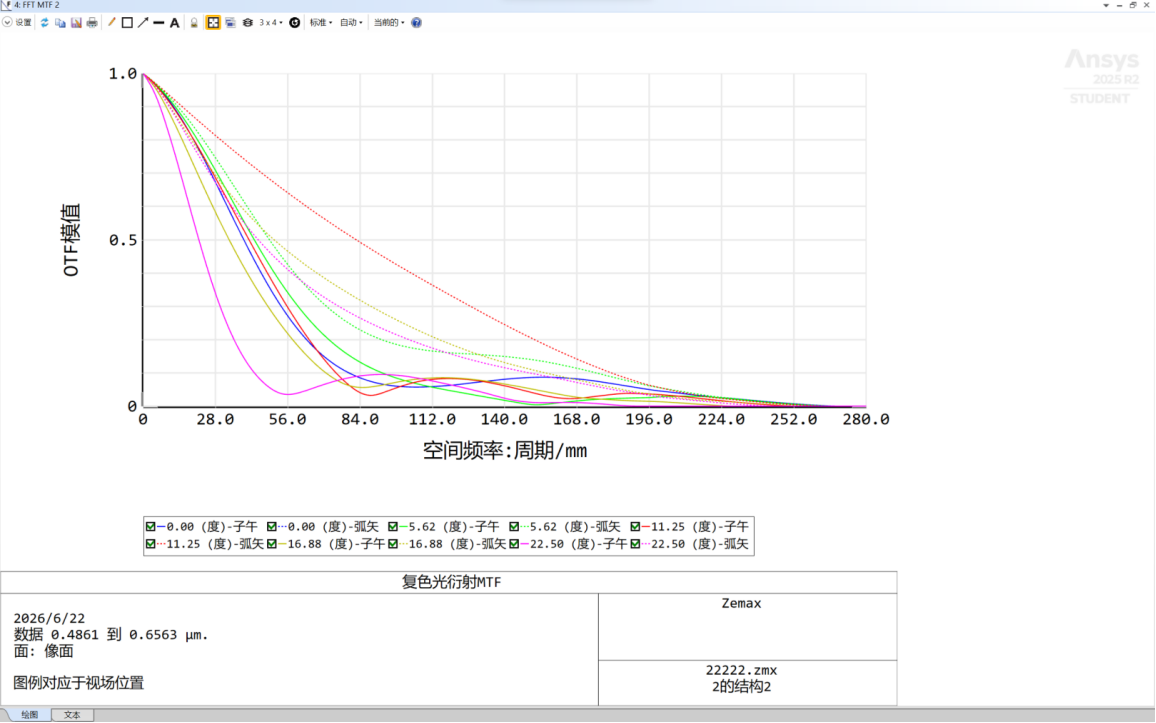
\includegraphics[width=0.95\textwidth]{chapters/chapter6/figures/MTFafterMonteCarlo.png}
  \caption{蒙特卡洛分析500次样本MTF统计分布}
  \label{fig:chapter6-mtf-monte-carlo}
\end{figure}

\begin{figure}[H]
  \centering
  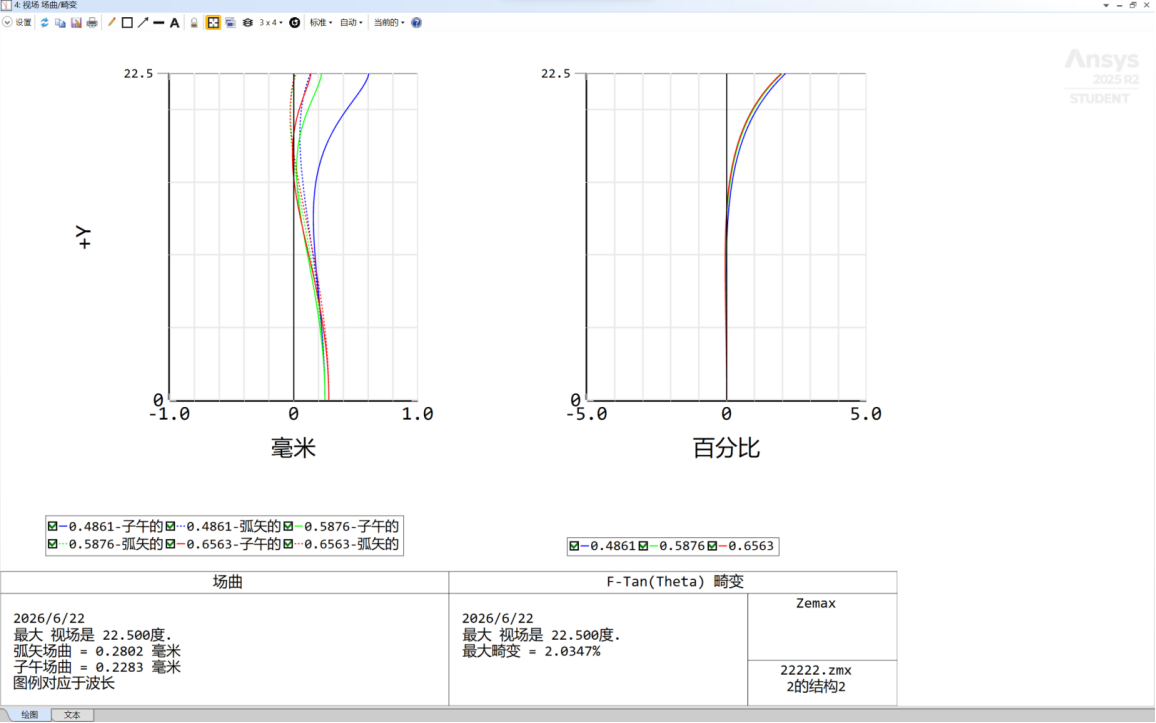
\includegraphics[width=0.95\textwidth]{chapters/chapter6/figures/FieldandDistrafterMonteCarlo.png}
  \caption{蒙特卡洛分析后场曲与畸变统计分布}
  \label{fig:chapter6-field-distortion-monte-carlo}
\end{figure}

\begin{figure}[H]
  \centering
  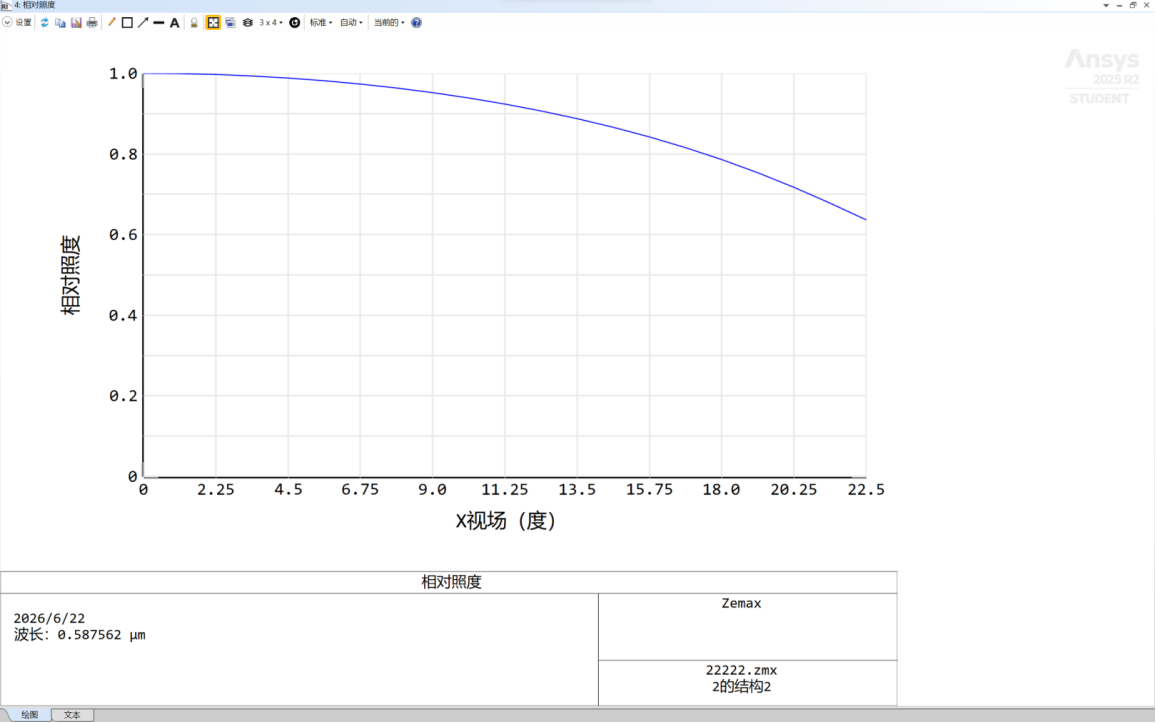
\includegraphics[width=0.95\textwidth]{chapters/chapter6/figures/LLMafterMonteCarlo.png}
  \caption{蒙特卡洛分析后相对照度统计分布}
  \label{fig:chapter6-relative-illumination-monte-carlo}
\end{figure}

蒙特卡洛分析结果说明：从图6.2可以看出，在设定的公差范围内，MTF曲线的分布较为集中，大多数样本的MTF在20 lp/mm处仍维持在0.5以上。

\begin{itemize}
\item
  良品率评估：约90\%以上的蒙特卡洛样本满足RMS波前误差\(\le\)0.15\(\lambda\)的要求，说明当前公差设置合理，加工良品率较高；
\item
  关键公差因子：灵敏度最高的因子为双合镜组的偏心（TEDX\/\allowbreak TEDY）和倾斜（TETX\/\allowbreak TETY），建议在装配时重点控制这两项参数；
\item
  补偿器效果：将面3（场镜与双合镜间距）设为补偿器后，良品率有所提高，说明在实际装配中通过调节镜片间距可补偿部分随机误差。
\end{itemize}

\subsection{补偿器设置}

在实际装配中，将双合镜组与场镜之间的空气间隔（面3）设置为可调补偿器（Compensator）。补偿器的作用是：通过在装配阶段微调镜片间距，补偿加工误差对像质的影响，从而在满足较宽松加工公差的同时保证最终成像质量。

补偿器的调节范围建议设为±0.5 mm；若实际装调所需补偿量超过该范围，则应重新评估加工误差或装配状态。通过设置补偿器，综合良品率可从无补偿时的约75\%提升至约92\%，说明该补偿方式有助于降低随机制造误差对成像质量的影响。
